\chapter{Dokumentace}

Vytvořili jsme Javascript knihovnu napsanou v jazyce Typescript, která nabízí
jednoduchý inteface pro vytváření programů usnadňující porovnání několika
sekundárních struktur RNA. V této kapitole odůvodníme volbu technologie
canvas\footnote{https://developer.mozilla.org/en-US/docs/Web/API/Canvas\_API}
pro vykreslování, seznámíme čtenáře s kódem, vstupními daty a v neposlední řadě
ukážeme, jak knihovnu používat.

\section{Použití canvasu} \label{canvas}

\subsection{Knihovna D3.js}

D3.js\footnote{https://d3js.org/} je knihovna v jazyce Javascript pomáhající
přivést data k životu podporující především
SVG\footnote{https://developer.mozilla.org/en-US/docs/Web/SVG}. SVG je webový
standard, který lze skvěle kombinovat s ostatními standardy jako je CSS,
DOM\footnote{https://developer.mozilla.org/en-US/docs/Web/API/Document\_Object\_Model},
Javascript.

D3.js knihovna klade důraz na webové standardy a tím dává uživateli možnost
využívat moderní prohlížeče naplno bez dalších frameworků. S knihovnou není
nejjednodušší se naučit pracovat, ale její velkou předností je rychlost a
široká paleta funkcí pro vizualizace dat.

\subsection{SVG}

V počátcích jsme chtěli k zobrazování používat SVG, které V kombinací s D3.js
knihovnou je velmi silný a flexibilní nástroj.

Bohužel SVG je poměrně pomalé a je to poznat už při vykreslování tisícovek
objektů. Takového počtu objektů můžeme dosáhnout pouze s jednou sekundární RNA
strukturou, protože každá čára je jeden objekt a každý nukleotid se vykresluje
jako dva objekty. My navíc chceme zobrazit více takových struktur a ještě s
nimi dynamicky pracovat. Tím se pro nás stalo SVG nepoužitelné.

\subsection{Canvas}

Další možností bylo využití canvasu, který slibuje výrazně lepší výkon a lze ho
stále jednoduše používat. Některé pro nás klíčové funkce D3.js knihovny lze
využít i pro práci s canvasem. Konkrétně se jedná o zoom, posouvání a animace.
U canvasu jsme nakonec i zůstali, přestože při práci s desítkami velkých
struktur vykreslování není plynulé.

\section{Struktura vstupních dat}

Výstupem nástroje Traveler jsou data ve formátu JSON, obsahující všechny
potřebné informace o rozložení nukleotidů, jejich párování, velikosti popisků,
barvách a tloušťkách čar. Kromě informací o rozložení lze z nich také vyčíst
informace o potřebných editacích vzorové sekundární struktury. Výstupní data
nástroje Traveler slouží jako vstupní data naší knihovny, proto podrobněji
popíšeme jejich strukturu.

RNA je sekvence nukleotidů, to znamená, že každý nukleotid má svůj index
(pořadí). V popisovaných datech je uložený index i jméno (A, C, G nebo U) pro
každý nukleotid. Kromě vlastního indexu a jména je u nukleotidu $n$ uložené i
jméno a index vzorového nukleotidu $v$ neboli index a jméno nukleotidu $v$ ve
vzorové struktuře, ze kterého lze nukleotid $n$ pomocí nějaké ze zmíněných
editací získat. Přidaný nukleotid je nukleotid, který nevznikl modifikací
nějakého nukleotidu ve vzorové struktuře a takový nukleotid má index vzorového
nukleotidu $-1$. Za pomocí těchto informací lze jednoduše zjistit, jestli je
nukleotid přidaný nebo přejmenovaný a pokud máme k dispozici i data vzorové
struktury, lze pomocí indexu porovnávat jejich souřadnice.

V rámci R2DT projektu vzniká JSON
schéma\footnote{https://github.com/LDWLab/RNA2D-data-schema}, které by mělo
popisovat strukturu vstupních dat. Schéma je stále ve vývoji, proto aktuální
výstupy Traveleru se mírně liší od schématu a je dost možné, že se formát
výstupu bude v budoucnu ještě měnit a naše knihovna se jim bude přizpůsobovat.

Samotná struktura dat není složitá, ale popíšeme zde pouze tu část, kterou
aktuálně využíváme, kromě toho, že ostatní data pro nás nejsou důležitá, tak
jak již bylo zmíněno samotná struktura dat není pevně daná a může se měnit.

Jedná se o objekt, který má dvě položky - \texttt{rnaComplexes} a
\texttt{classes}, což je pole objektů popisující třídy říkající způsob
zobrazení struktury, podobně jako to kaskádové
styly\footnote{https://developer.mozilla.org/en-US/docs/Web/CSS} (CSS) diktují
pro webové stránky. 

\texttt{rnaComplexes} je pole polí sloužící pro popis celých skupin RNA
struktur. Naše knihovna pracuje vždy pouze s nultým prvkem. Neviděli jsme důvod
to dělat jinak, a pokud by se nějaký důvod našel v budoucnu, neměl by být
problém naší knihovnu přizpůsobit situaci (např. rozšířením o novou metodu pro
zachování zpětné kompatibility).

V rámci naší knihovny jsme vytvořili interface, který vstupní data musí
splňovat. Struktura zbytku dat by měla být jasně viditelná z diagramu
\ref{datainter} těchto interfaců.

\begin{figure}[H]
  \centering
  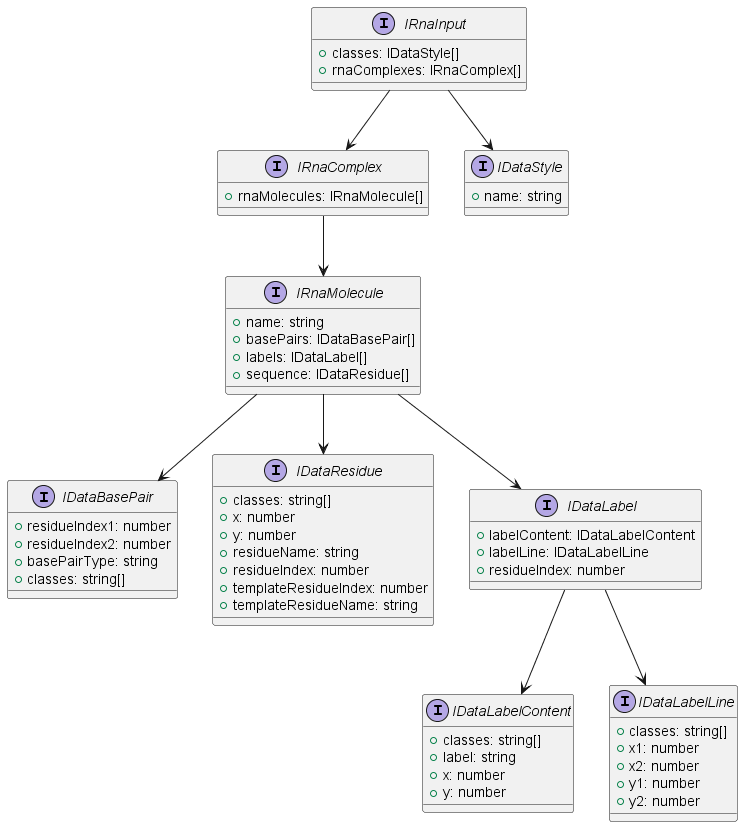
\includegraphics[width=145mm]{../img/kap03/rnaInput.png}
  \caption[Interface pro vstupní data]{Interface pro vstupní data.}
  \label{datainter}
\end{figure}

\section{Objektový návrh}

V následující části se pokusíme čtenáře seznámit s objektovým návrhem naší
knihovny. V této části dáme obecný pohled na strukturu tříd a později i ukážeme
jak se s třídami dá pracovat.

Srdcem celé knihovny je třída \texttt{RnaVis}. Má v sobě uložené vrstvy
realizované třídou \texttt{Layer}, představující jednotlivé struktury. Třída
\texttt{RnaVis} vykresluje struktury na canvas, nastavuje se přes ní
zoom/posouvání a zpřístupňuje většinu funkcionality.

Pro určení vykreslovacích parametrů (např. font, barva, velikost) objektů  máme
třídu \texttt{Styles}. Před každým vykreslením se zeptáme této třídy na
vykreslovací parametry pro daný objekt. Důvod, proč jsme zvolili takovéhle
řešení problému je, že jsme původně neměli jasnou představu, co a jak bude
řešené, a proto nám přišlo nejjednodušší tuto část oddělit a použít stejný
způsob, jaký se používá ve vstupních datech.

Poslední důležitou velkou částí jsou animace. Tuto funkcionalitu zpřístupňují
dvě hlavní třídy - \texttt{TranslationAnim}, \texttt{VisibilityAnim}. Obě
implementují interface \texttt{IAnimation}. 

\sloppy

Diagramy tříd \ref{diagram1}, \ref{diagram2}, \ref{diagram3} dohromady obsahují
každou třídu. Diagramama se snažíme vyjádřit obecnou strukturu, tím pádem pro
přehlednost neobsahují všechny informace - všechny metody, některé privátní
vlastnosti a některé závislosti. Pro podrobnější rozbor tříd a metod se
doporučujeme podívat do referenční
dokumentace\footnote{https://github.com/michalhercik/rna-visualizer/blob/main/lib/docs/README.md}.

\fussy
 
\begin{figure}[H]
  \centering
  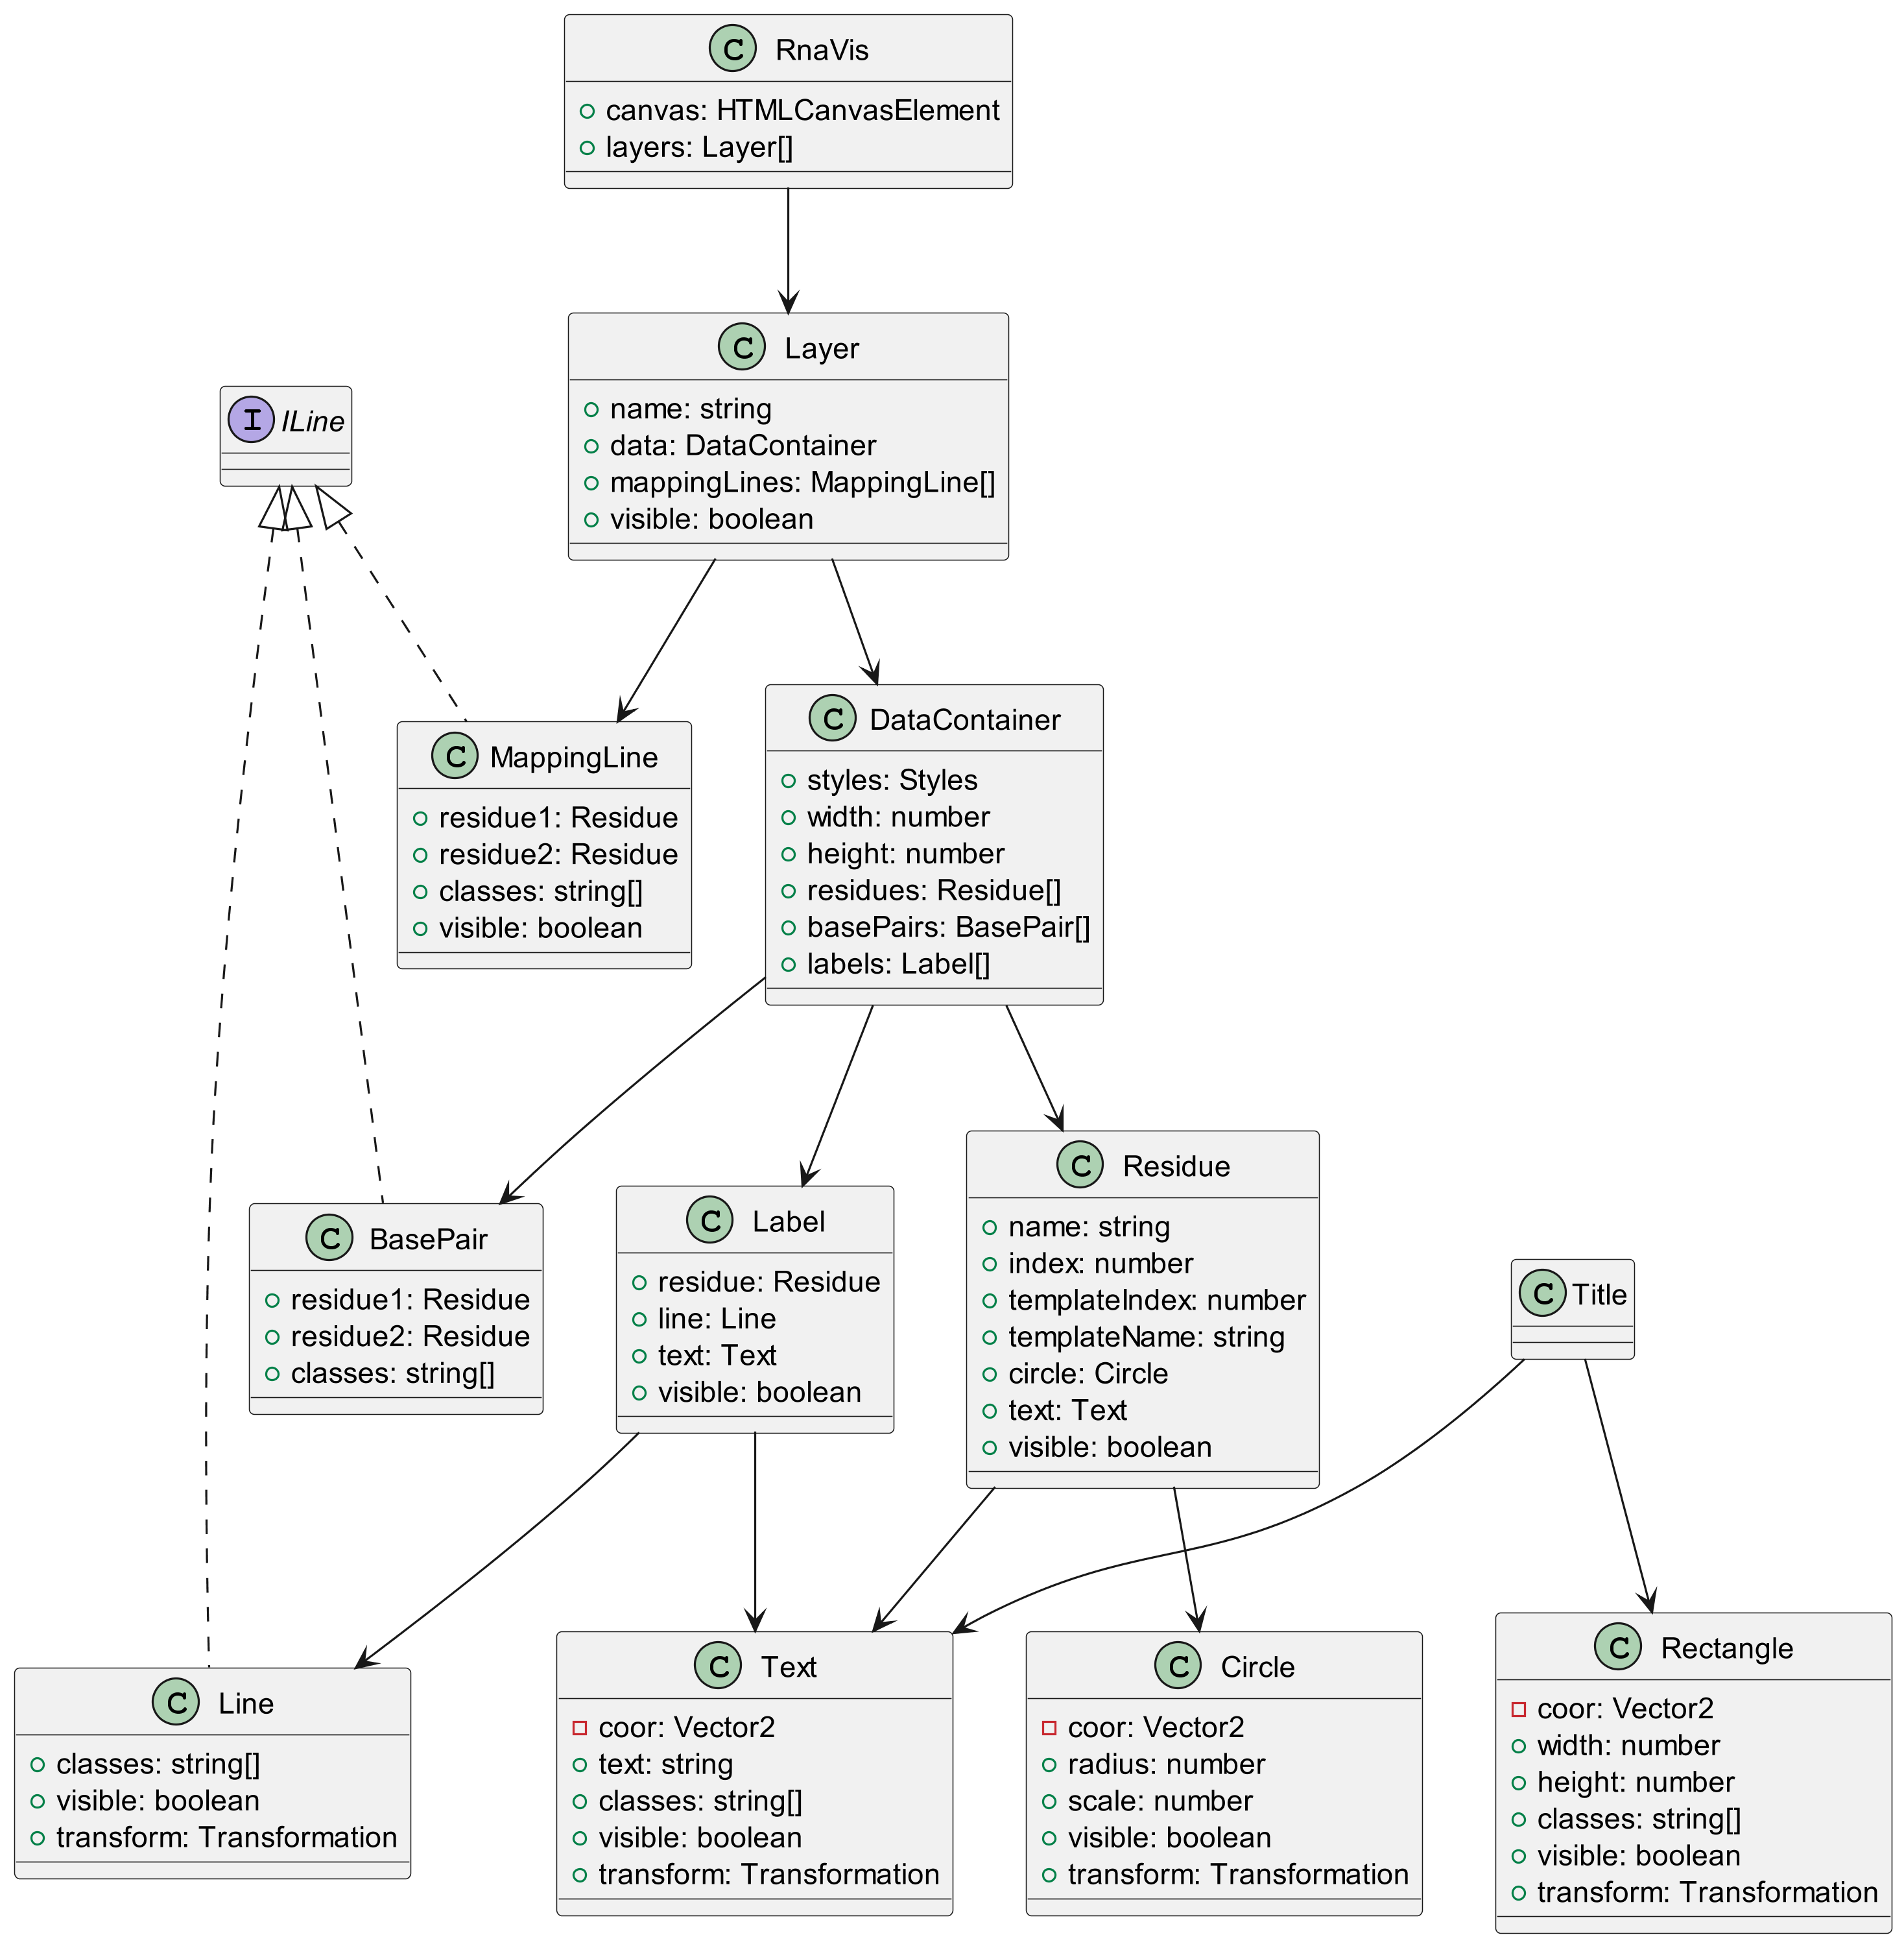
\includegraphics[width=145mm]{../img/kap03/rnavis.png}
  \caption[Diagram tříd]{Diagram tříd.}
  \label{diagram1}
\end{figure}

\begin{figure}[H]
  \centering
  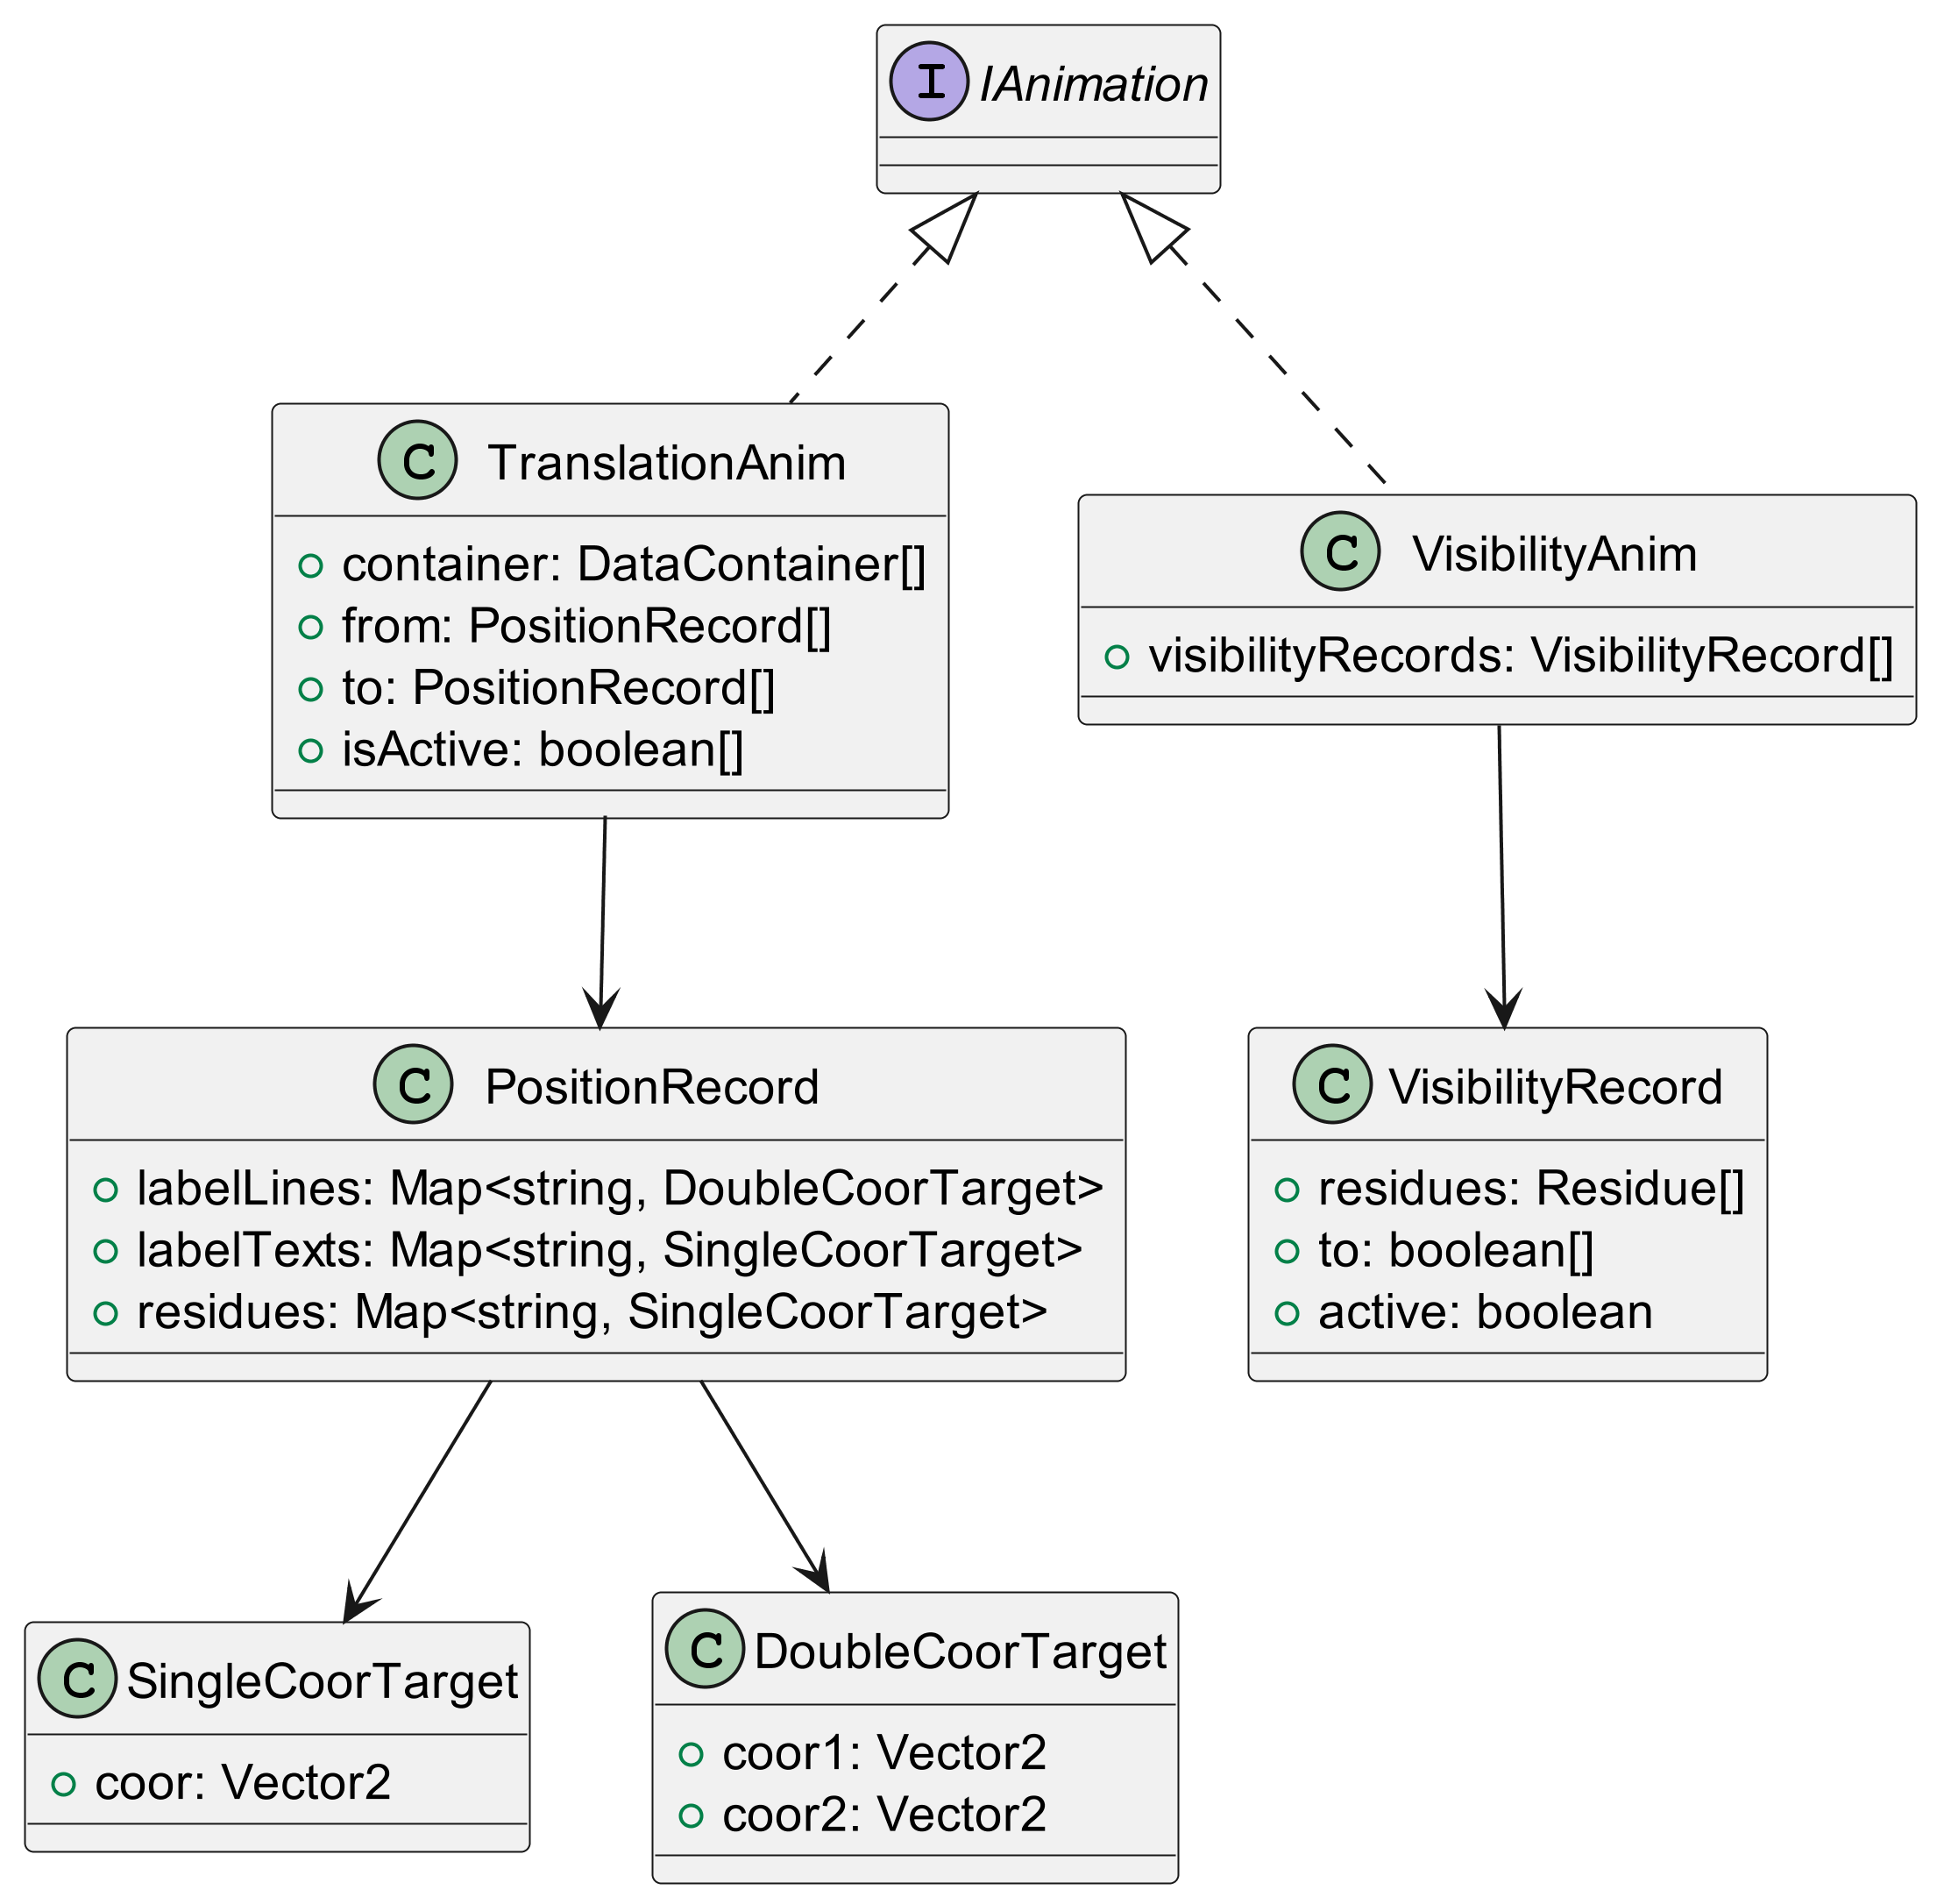
\includegraphics[width=145mm]{../img/kap03/animation.png}
  \caption[Diagram tříd]{Diagram tříd.}
  \label{diagram2}
\end{figure}

\begin{figure}[H]
  \centering
  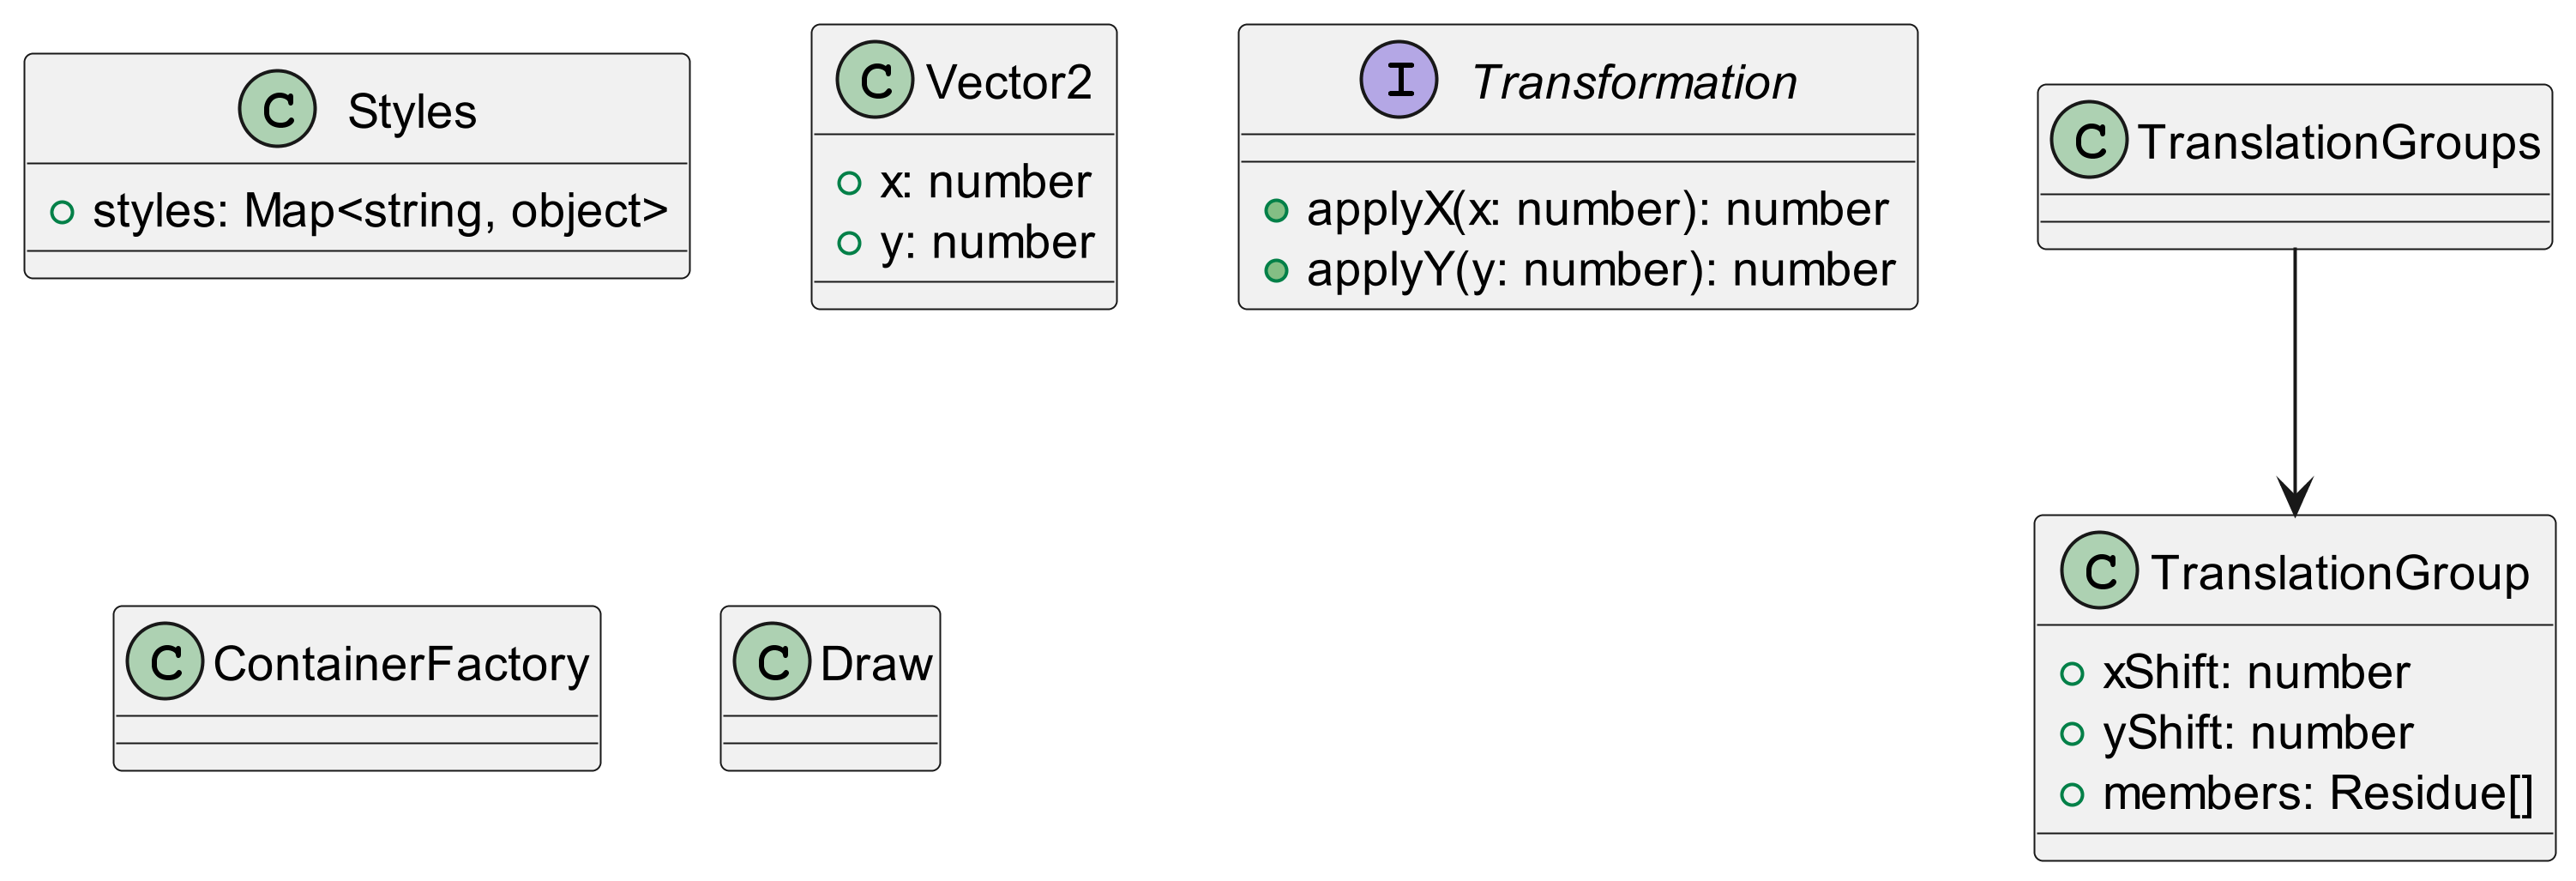
\includegraphics[width=145mm]{../img/kap03/others.png}
  \caption[Diagram tříd]{Diagram tříd.}
  \label{diagram3}
\end{figure}

\section{Uživatelské seznámení s knihovnou} \label{seznameni}

S obecnou strukturou kódu jsme čtenáře seznámili a nyní ukážeme, jak lze
knihovnu užívat. Bude se jednat o ukázku implementací základních využití, jako
je vykreslení struktur, zarovnání, transformace na vzorovou strukturu a některé
další možnosti. Knihovna je dostupná přes
npm\footnote{https://www.npmjs.com/package/rna-visualizer} nebo na
GitHub\footnote{https://github.com/michalhercik/rna-visualizer}.

\subsection{Vytvoření objektu RnaVis a vykreslení struktur}

V prvním kroce importujeme veškeré potřebné zdroje\ref{import}. Použité vstupní data
\texttt{d.5.b.A.madurae.json} a \texttt{URS00000B9D9D.json} jsou dostupné na
GitHub stránce
projektu\footnote{https://github.com/michalhercik/rna-visualizer/blob/main/demo/example\_data/madurae\\/URS00000B9D9D\_471852-d.5.b.A.madurae.json}
\footnote{https://github.com/michalhercik/rna-visualizer/blob/main/demo/example\_data/madurae\\/d.5.b.A.madurae\_fromn\_d.5.b.A.madurae.colored.json}

\begin{lstlisting}[caption={Import},label=import]
import { 
  RnaVis, 
  TranslationGroups, 
  PositionRecord,
  TranslationAnim,
} from 'rna-visualizer';
import template from './d.5.b.A.madurae.json';
import structure from './URS00000B9D9D.json';
\end{lstlisting}

Následně vytvoříme \texttt{canvas}, na který budeme vykreslovat, nastavíme mu
šířku, výšku a přidáme ho do těla dokumentu\ref{tscanvas}.

\begin{lstlisting}[caption={Vytvoření a nastavení canvas},label=tscanvas]
const canvas = document.createElement('canvas');
canvas.width = 500;
canvas.height = 500;
document.body.appendChild(canvas);
\end{lstlisting}

Nyní už můžeme vytvořit samotný objekt \texttt{RnaVis}\ref{rnavis}, který nás bude provázet
v ostatních ukázkách.

\begin{lstlisting}[caption={Vytvoření RnaVis}, label=rnavis]
const rnaVis = new RnaVis(canvas);
\end{lstlisting}

Přidáme do něj dvě struktury - \texttt{template} a \texttt{structure}\ref{vrstvy}.
Struktury se přidávají pomocí metody \texttt{addLayer}, která má tři parametry
- přidávanou strukturu, libovolný název a poslední třetí parametr je volitelný
a slouží k určení, jestli chceme, aby se struktura vykreslovala a jeho
defaultní hodnota je \texttt{true}, tedy defaultně se struktura vykresluje.
Knihovna předpokládá, že první přidaná struktura, je vzorová struktura, ze
které jsou všechny ostatní vygenerované.

\begin{lstlisting}[caption={Přidání struktur}, label=vrstvy]
rnaVis
  .addLayer(template, 'd.5.b.A.madurae')
  .addLayer(structure, 'URS00000B9D9D');
\end{lstlisting}

Struktury lze potom vykreslit pomocí metody \texttt{draw}\ref{draw}.

\begin{lstlisting}[caption={Vykreslení struktur}, label=draw]
rnaVis.draw();
\end{lstlisting}

Celý kód lze zapsat následovně\ref{shrnuti}.

\begin{lstlisting}[caption={Celý kód pohromadě}, label=shrnuti]
import { 
  RnaVis, 
  TranslationGroups, 
  PositionRecord,
  TranslationAnim,
} from 'rna-visualizer';
import template from './d.5.b.A.madurae.json';
import structure from './URS00000B9D9D.json';

const canvas = document.createElement('canvas');
canvas.width = 500;
canvas.height = 500;
document.body.appendChild(canvas);

new RnaVis(canvas)
  .addLayer(template, 'd.5.b.A.madurae')
  .addLayer(structure, 'URS00000B9D9D')
  .draw();
\end{lstlisting}

V dalších ukázkách budeme předpokládat předchozí kroky a budeme na ně
navazovat.

\subsection{Zoom a posouvání canvasu}

Pro přidání zoomu a posouvání stačí zavolat metodu \texttt{addZoom} na instanci
třídy \texttt{RnaVis}\ref{zoom}, která přidá obě funkcionality canvasu
předanému jako parametr konstruktoru objektu. Interně používá metoda D3.js
knihovnu pro zpracování zoom a posunutí canvasu.

\begin{lstlisting}[caption={Přidání zoom a posouvání}, label=zoom]
rnaVis.addZoom();
\end{lstlisting}

\subsection{Zarovnání struktur}

Zarovnání struktur\ref{zarovnani} docílíme tak, že zavoláme na instanci třídy \texttt{RnaVis}
metodu \texttt{align}, která vrátí pole objektů typu \texttt{Vector2}, které
reprezentují posunutí pro každou strukturu. Následně zavoláme na instanci třídy
\texttt{RnaVis} metodu \texttt{translate}, které předáme pole obsahující
posunutí a metoda posune každou strukturu o příslušné posunutí. Potom už stačí pouze vykreslit struktury metodou \texttt{draw}\ref{tsalign}.

\begin{lstlisting}[caption={Zarovnání struktur}, label=tsalign]
const translations = rnaVis.align();
rnaVis
  .translate(translations);
  .draw();
\end{lstlisting}

\subsubsection{Zarovnání struktur na konkrétní skupinu}

Metoda \texttt{align} má volitelný parametr typu \texttt{number}, kterým můžeme
vybrat, na kterou skupinu nukleotidů chceme dostat zarovnání\ref{groupalign}.

Při první iteraci se porovnává první přidaná struktura (vzorová) s druhou
přidanou strukturou a roztřídí se nukleotidy podle posunutí, které je zarovná.
Číselný parametr potom určuje, která skupina se použije pro filtrování v
dalších iterací. 

Pokud je parametr prázdný nebo menší než nula, vybere se největší skupina.
Pokud je parametr větší, než počet vytvořených skupin metoda vyhodí výjimku se
zprávou \texttt{groupIndex >= groups.length}. 

V následující ukázce vytvoříme skupiny, které vzniknout při první iteraci a
vybereme nejmenší, kterou pak použijeme pro zarovnání struktur. Skupiny
vytvoříme statickou metodou \texttt{TranslationGroups.create}. První parametr
je vzorová struktura, druhý parametr je struktura, kterou chceme zarovnat.
Třetí parametr jsou skupiny pomocí, kterých chceme filtrovat a je volitelný a
poslední parametr je minimální velikost výstupních skupin, který je taky
volitelný a jeho defaultní hodnota je $5$.

\begin{lstlisting}[caption={Zarovnání struktur na skupinu nukleotidů}, label=groupalign]
const containers = rnaVis.getDataContainers();
const groupSizes = 
  TranslationGroups.create(containers[0], containers[1], null, 20)
  .map(group => group.size());
const groupIndex = groupSizes.indexOf(Math.min(...groupSizes));
const translationsToGroup = rnaVis.align(groupIndex);
rnaVis
  .translate(translationsToGroup)
  .draw();
\end{lstlisting}

\subsubsection{Zarovnání na nukleotid}

Zarovnání na nukleotid obsahuje podobné kroky. Nejdřív si zvolíme nukleotid ze
vzorové struktury, na který chceme struktury zarovnávat. Potom na instanci
třídy \texttt{RnaVis} pomocí metody \texttt{getAlignmentToTempResidue} získáme
posunutí pro každou strukturu a nakonec struktury zarovnáme a vykreslíme\ref{resalign}.

\begin{lstlisting}[caption={Zarovnání struktur na nukleotid}, label=resalign]
const templateResidue = rnaVis.layers[0].data.residues[42];
const translationsToResidue = 
  rnaVis.getAlignmentToTempResidue(templateResidue);
rnaVis
  .translate(translationsToResidue)
  .draw();
\end{lstlisting}

\subsubsection{Animace zarovnání}

Jakýkoliv přechod je pro oko vždy příjemnější animovat a to knihovna umožňuje
pomocí jednoduchého rozhraní pro animace. V následující ukázce ukážeme jak
animovat zarovnání struktur.

V prvním kroce vytvoříme pro každou strukturu \texttt{PositionRecord}, který
obsahuje pozice nukleotidů a popisků. V tomto případě bude obsahovat cílovou
pozici pro každý nukleotid a vytvoříme ho pomocí statické metody
\texttt{fromTranslation}, která bere jako parametr strukturu a posunutí
struktury.

Následně vytvoříme objekt typu \texttt{TranslationAnim}, který umožňuje mimo
jiné animovat transformaci struktury na daný \texttt{PositionRecord}. Potom už
jenom zavoláme metodu \texttt{animate}, kterou začne celá animace. Jako
parametry bere instanci třídy \texttt{RnaVis}, kterou používá pro vykreslování
každého snímku animace, trvání animace v milisekundách a poslední volitelný
parametr je funkce, která se zavolá na konci animace. V ukázce na konci animace
jí otočíme a animujeme zpátky do původního stavu\ref{animalign}.

\begin{lstlisting}[caption={Animace zarovnání}, label=animalign]
const containers = rnaVis.getDataContainers();
const animationTargets = rnaVis
  .align()
  .map((translation, i) 
    => PositionRecord.fromTranslation(containers[i], translation)
  );

const anim = new TranslationAnim(containers, animationTargets);
anim.animate(rnaVis, 1500, () => {
  anim.reverse();
  anim.animate(rnaVis, 1500);
});
\end{lstlisting}

\subsection{Mapovací čáry}

Zobrazení čar, které ukazují mapování nukleotidů, je velmi jednoduché.
Mapovací čáry se vytvoří hned při přidání každé vrstvy a jsou defaultně
schované, proto je stačí pouze zviditelnit\ref{map}.

\begin{lstlisting}[caption={Zobrazení mapovacích čar}, label=map]
rnaVis.layers.forEach(
  l => l.mappingLines.forEach(
    m => m.setVisible(true)
  )
);
rnaVis.draw();
\end{lstlisting}

\subsection{Transformace na vzorovou strukturu}

Poslední ukázkou je transformace na vzorovou strukturu. V ukázce nejdříve
schováme nukleotidy, které nemají vzorový nukleotid. Potom vytvoříme opět
\texttt{PositionRecord}, tentokrát pomocí statické metody
\texttt{fromTemplate}, která každému nukleotidu dá pozici jeho vzorového
nukleotidu. Potom už jenom animujeme přechod\ref{transform}.

\begin{lstlisting}[caption={Transformace na vzorovou strukturu}, label=transform]
const containers = rnaVis.getDataContainers().slice(1);
const targetStructure = rnaVis.layers[0].data;

containers.forEach(c => {
  c.getUnmappableResidues().forEach(
    r => r.setVisible(false)
  );
});

const targets = containers.map(
  cont => PositionRecord.fromTemplate(cont, targetStructure)
);
new TranslationAnim(containers, targets)
  .animate(rnaVis, 1500);
\end{lstlisting}

\section{Demonstrace metod}

V rámci naší knihovny jsme vytvořili také webovou
aplikaci\footnote{https://michalhercik.github.io/rna-visualizer/}\ref{demobla},
která demonstruje možnosti naší knihovny. Tato aplikace umožňuje uživatelům
pracovat s jednotlivými metodami nebo se všemi metodami najednou pro usnadnění
porovnání - překládání se zarovnáním, transformace na vzorovou strukturu,
mapovací čáry a další možnosti pro zpříjemnění práce. 

\begin{figure}[H]
  \centering
  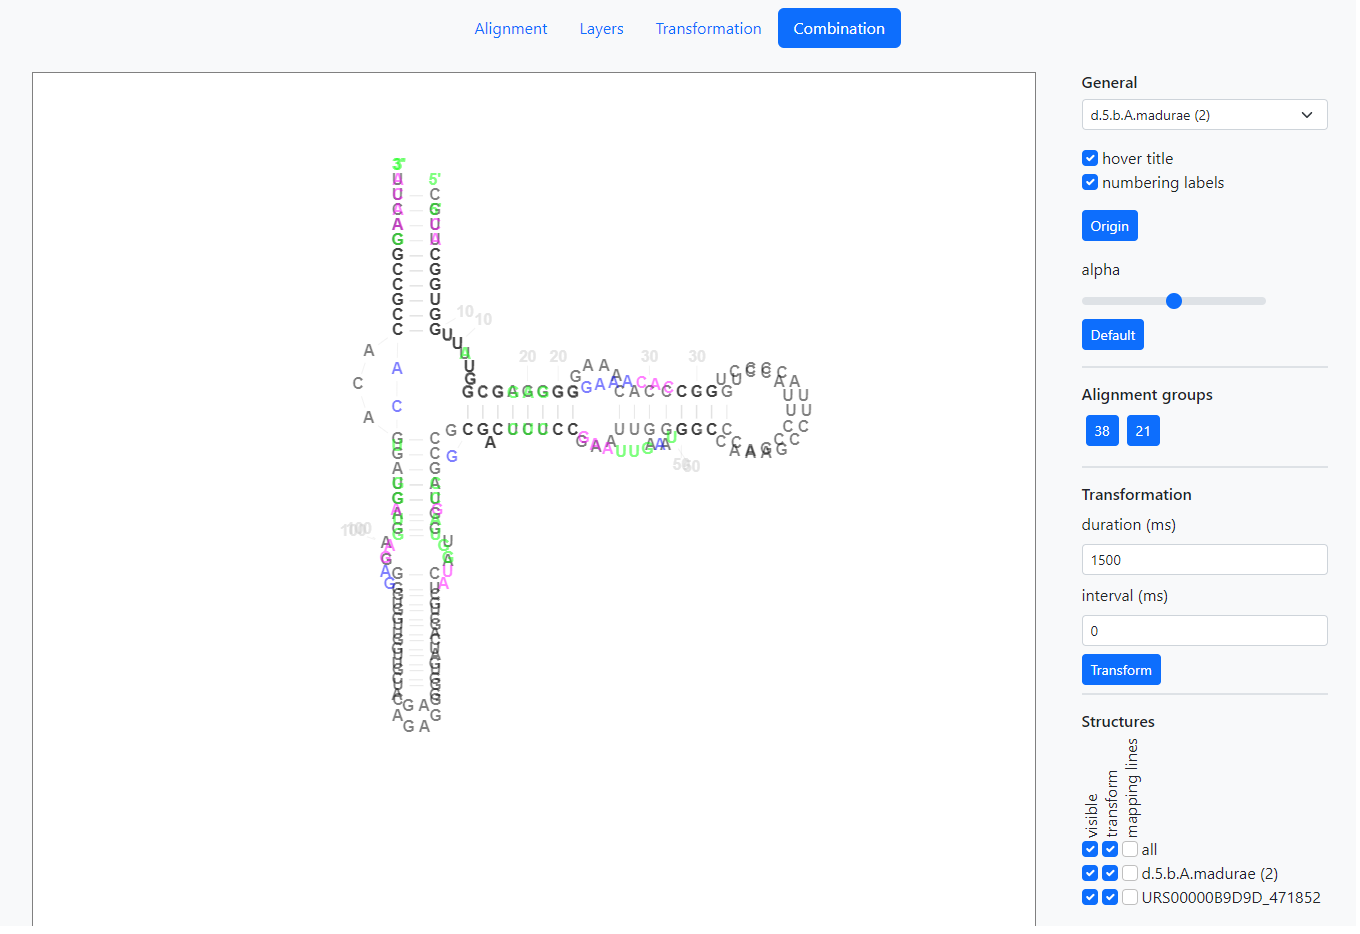
\includegraphics[width=145mm]{../img/kap03/demo.png}
  \caption[Snímek aplikace vytvořené pro demostraci funkcionality
  knihovny]{Snímek aplikace vytvořené pro demostraci funkcionality knihovny.}
  \label{demobla}
\end{figure}

\subsection{Získání testovacích dat}

\sloppy

Pro testování a demonstraci metod potřebujeme vstupní data, která budou
různorodá co do velikosti struktur tak do počtu. Zároveň potřebujeme, aby
vstupní data byla realistická, protože chceme řešit skutečné problémy.
Otevřená databáze RNAcentral používá ke generovaní sekundárních struktur RNA
nástroj R2DT\ref{r2dt}, proto jsou data z RNAcentral vhodným kandidátem.

Pro přístup k databázi lze použít jak API\footnote{https://rnacentral.org/api},
tak přímo posílat SQL
dotazy\footnote{https://rnacentral.org/help/public-database}. Databáze bohužel
nezpřístupňuje mapování nukleotidů na vzorovou strukturu, které nástroj R2DT
generuje, přesto je databáze užitečná a chybějící údaje lze dogenerovat.

Pro získání testovacích dat jsme využívali veřejný SQL přístup a celý postup
popisujeme v následujících bodech:
\begin{enumerate}
  \item Pomocí SQL dotazu\ref{vzorsql} jsme si zobrazili vzorové struktury a nějaké vybrali.
  \item Následně jsme pro každou vybranou vzorovou strukturu vybrali náhodně
    nejvýše $20$ RNA struktur, které použili danou vzorovou strukturui\ref{structsql}.
  \item Posledním krokem získáme mapovaní struktur na vzorovou strukturu.
    Použijeme R2DT s parametrem \texttt{--force\_template <template\_id>}, kde
    \texttt{template\_id} je identifikátor vzorové struktury, která je
    přiřazená generované struktuře v RNAcentral. Díky znalosti, kterou vzorovou
    strukturu použít, se přeskočí klasifikační kroky a celý proces se urychlý.
\end{enumerate}

\fussy
